\chapter{Tabele cu rezultate}


\chapter{Cod sursă}

\begin{figure}[h]
    \centering
    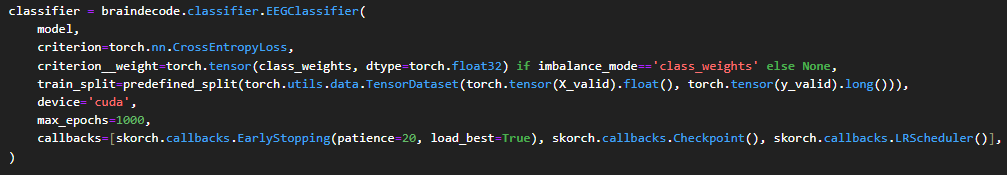
\includegraphics[width=1\linewidth]{wrapper_clasificator_braindecode.png}
    \caption{Apelarea wrapper-ului din braindecode}
    \label{fig:wrapper_braindecode}
\end{figure}

\begin{figure}[h]
    \centering
    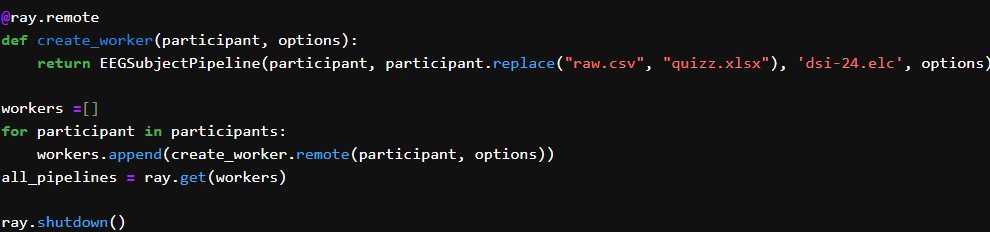
\includegraphics[width=1\linewidth]{images/ray.png}
    \caption{Paralelizare utilizând Ray}
    \label{fig:paralelizare_ray}
\end{figure}

\begin{figure}[h]
    \centering
    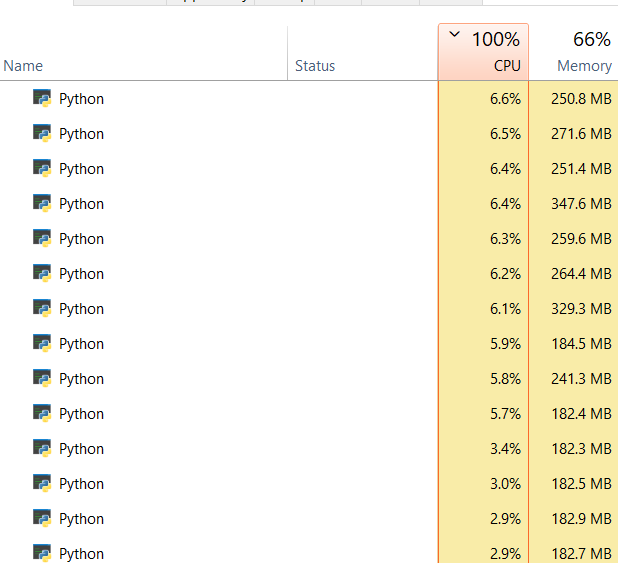
\includegraphics[width=0.7\linewidth]{task_manager.png}
    \caption{Load-ul pe calculator}
    \label{fig:load_calculator}
\end{figure}

\begin{figure}
    \centering
    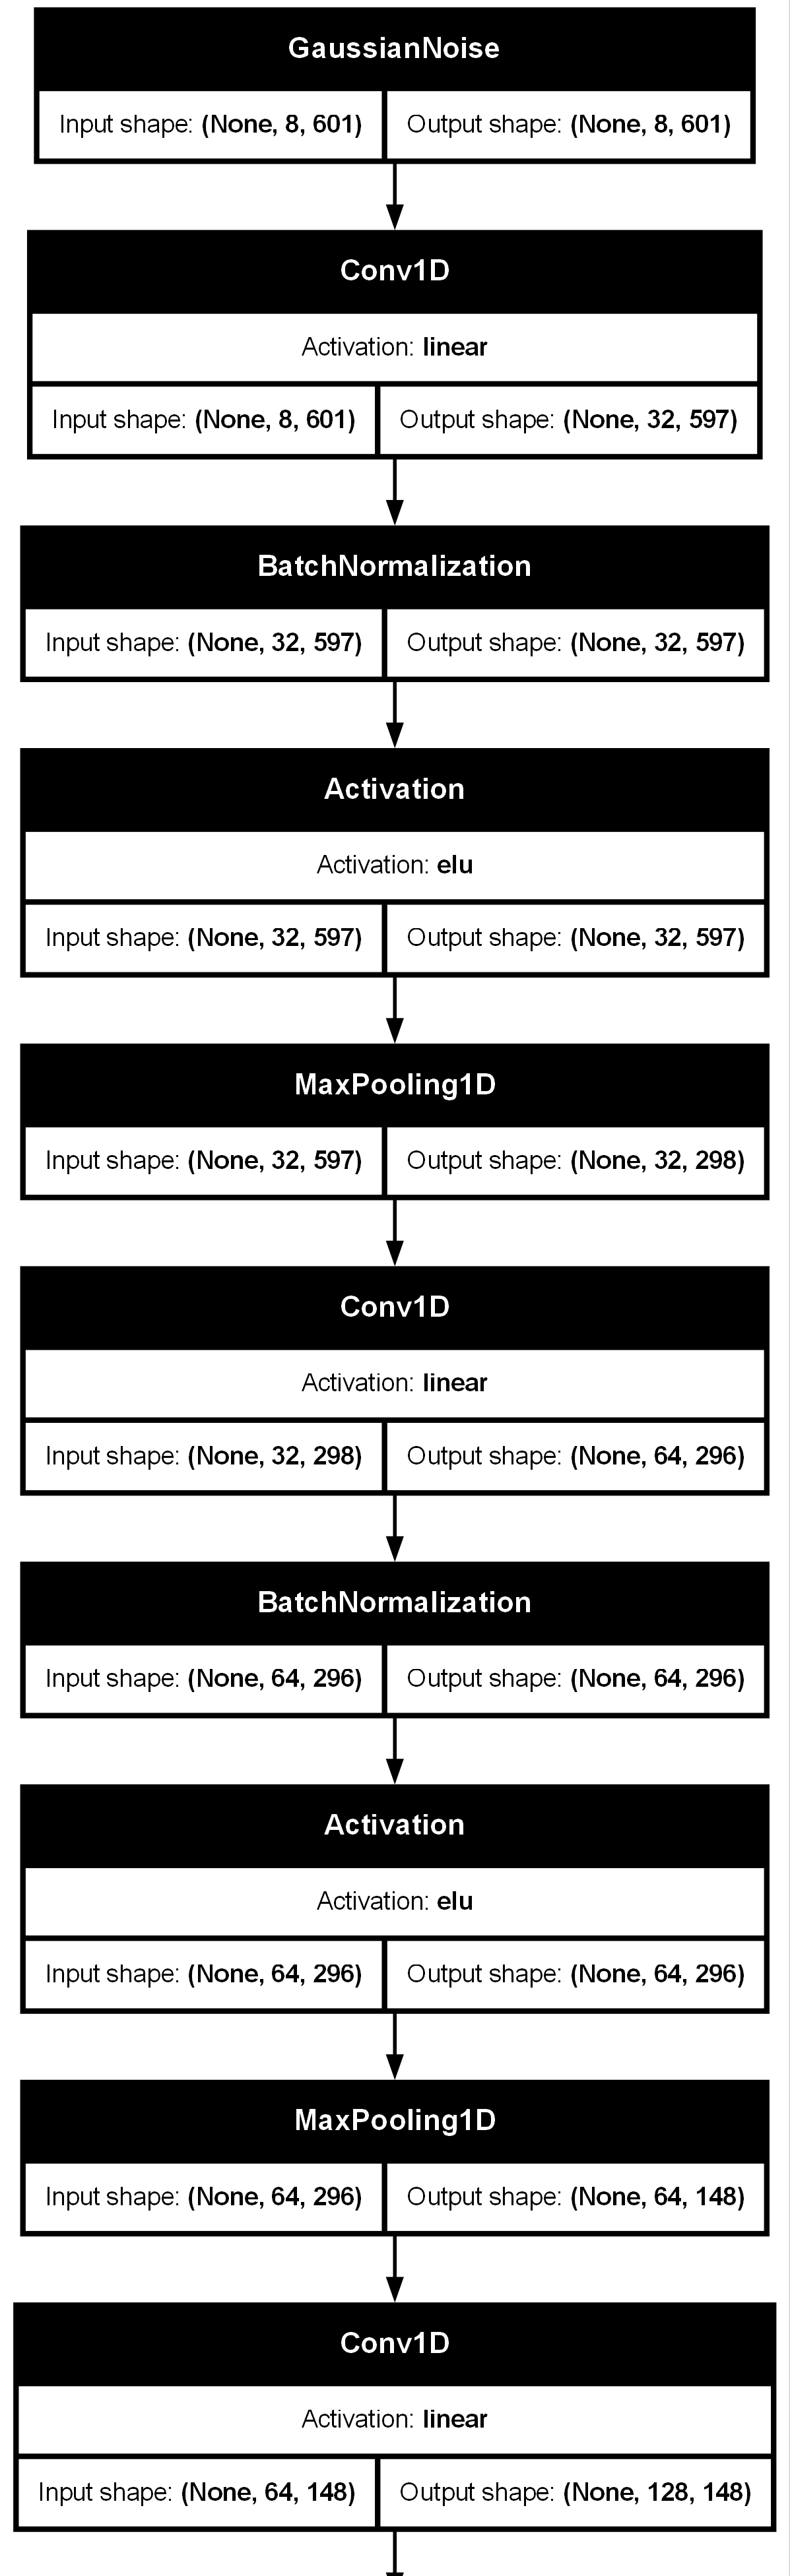
\includegraphics[width=0.4\linewidth]{model_part1.png}
    \caption{Model personal, partea 1}
    \label{fig:model_part1}
\end{figure}

\begin{figure}
    \centering
    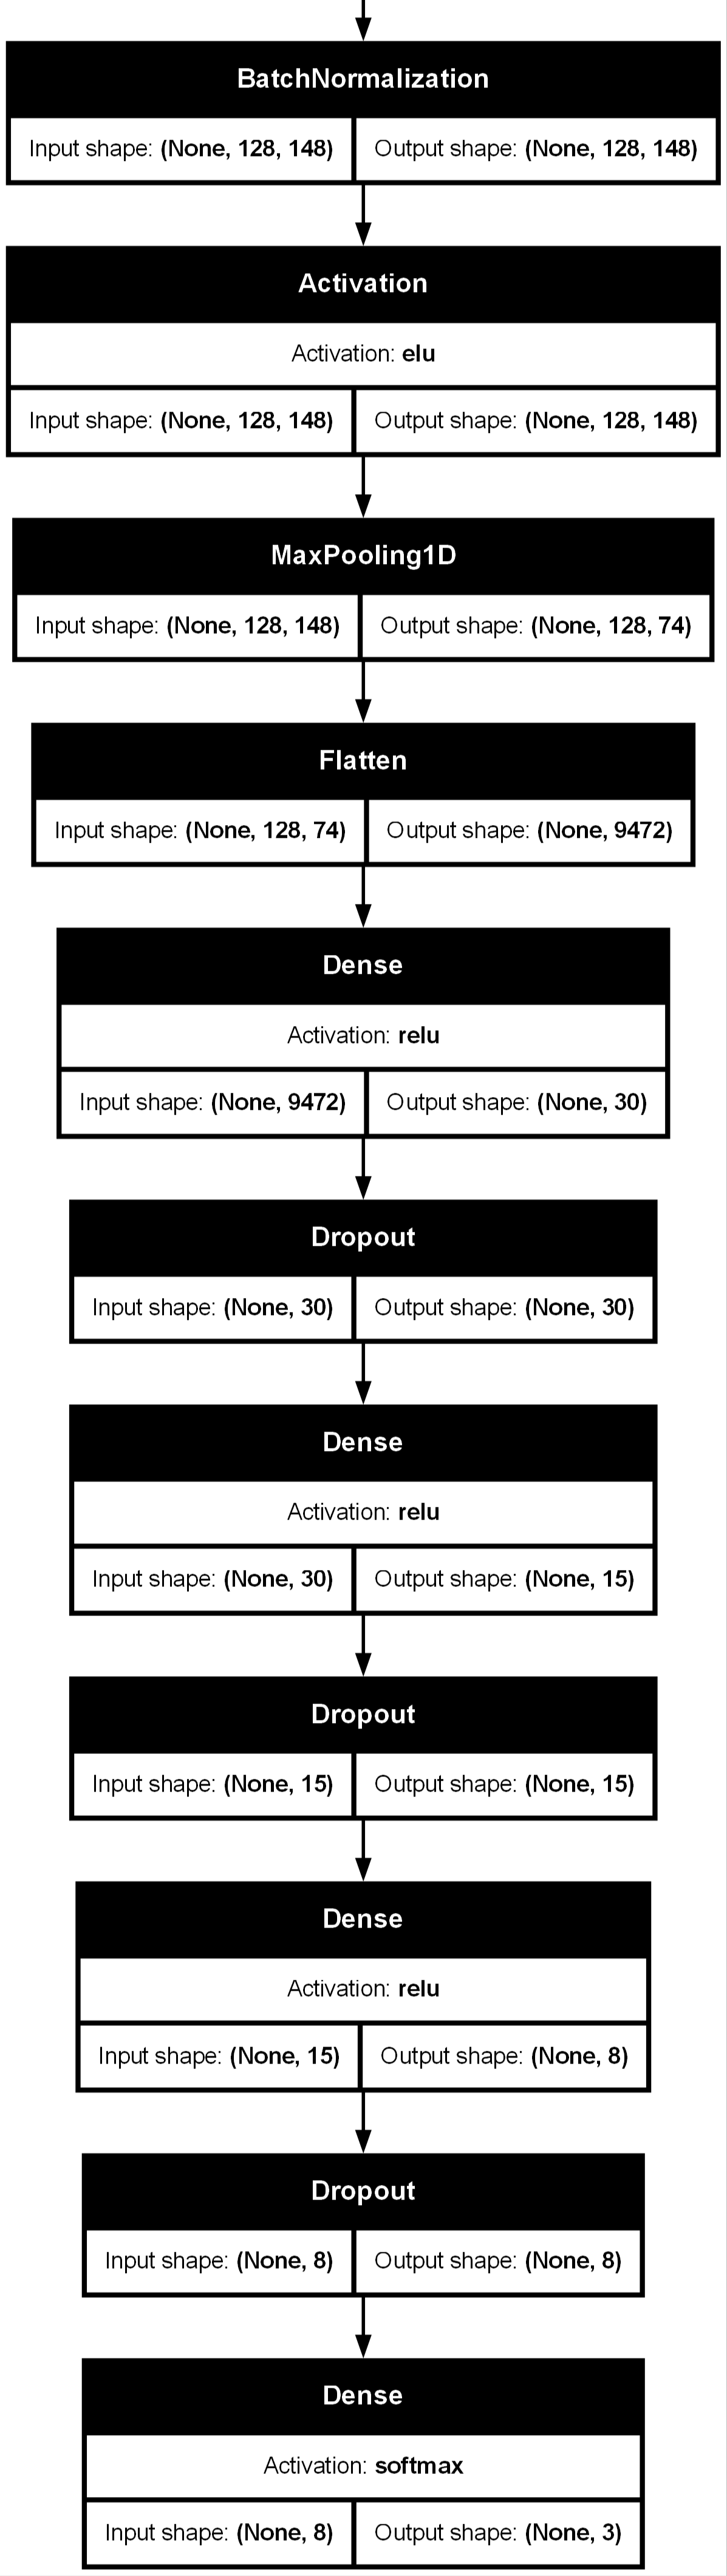
\includegraphics[width=0.4\linewidth]{model_part2.png}
    \caption{Model personal, partea 2}
    \label{fig:model_part2}
\end{figure}

\begin{figure}
    \centering
    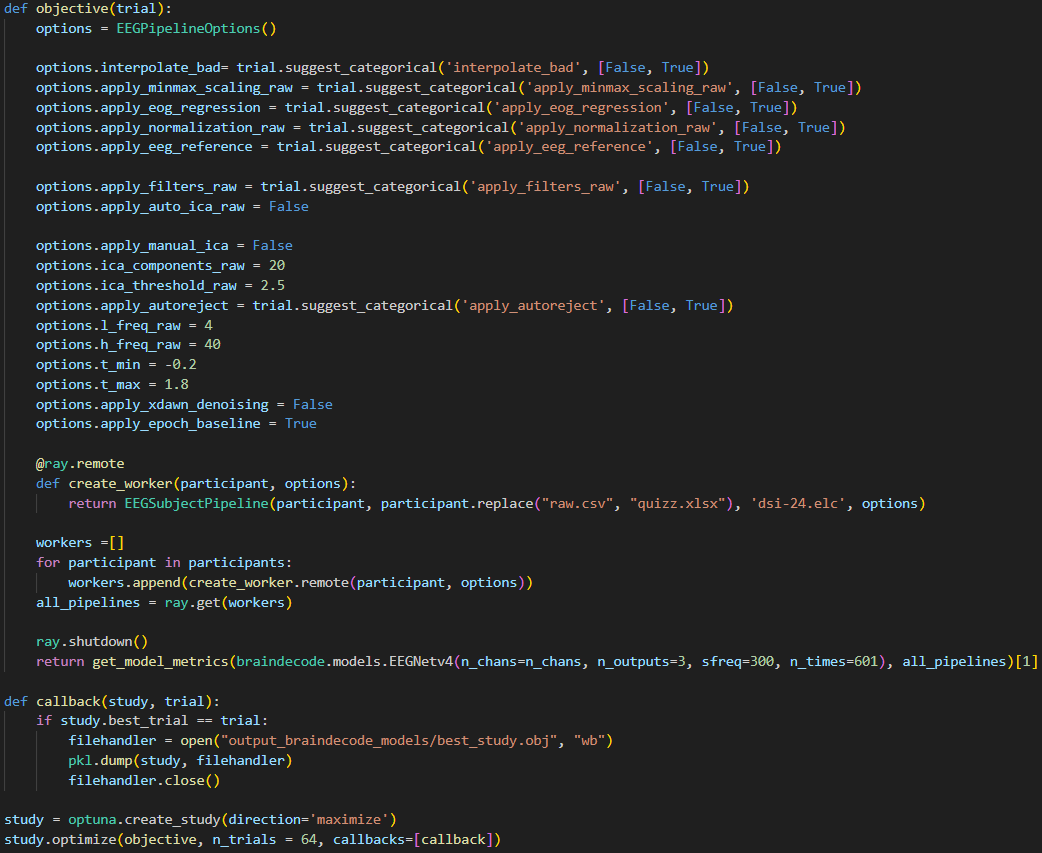
\includegraphics[width=1\linewidth]{optuna_study.png}
    \caption{Cautarea hiperparametrilor folosind optuna}
    \label{fig:optuna_search}
\end{figure}